\section{Cancer}
\label{intro-sec:cancer}

For a long time in human history, the origin of cancer as a disease was a mystery and a multitude of theories, starting in ancient Egypt, were developed. These theories ranged from a curse to chemical imbalance over parasites to trauma. Around 3000BC the Egyptians describe the bulging tumour of the breast as an incurable disease with no cure \cite{Breasted1930}, even then they already had some ointments, which were used, including resection, cauterisation and salting of the affected areas, all of which were still used up until the 19$^{th}$ century \cite{Hajdu2004}.

When the ancient Greeks laid the foundation for modern medicine with Hippocrates, the first hypothesis about natural causes of cancers was formulated and the terms ``cancer`` and ``carcinoma`` were coined. The abundance and accumulation of ``black bile`` in the body was thought to be the cause of the cancers. However, the treatment was still the same as before with resection and lotions \cite{Chadwick1950}.

Following Hippocrates, the Roman physician Celsus progressed the understanding of cancers significantly, by describing metastatic relapse of treated breast cancer in neighbouring armpits and even the spread to distant organs. He also was aware, that the outcome of patients was better, if the tumours were removed early and aggressively \cite{Celsus1939}.

With the destruction of the western Roman empire, the middle east became well known for their strong advances towards modern medicine and the court physician to the Emperor of Constantinople Aetius had success with the first total mastectomy and generally was an advocate of the total excision of tumours \cite{Browne2012}. 

Sadly, while both the understanding of cancer as well as the treatment were steadily improving, the Pope prohibited bloodshed as well as surgeries and therefore lead to a slow down of advances, especially because autopsies were also forbidden a hundred years later in 1305. However, there were still illegal experiments conducted and the general classification which is still used up to date was started, by Henri de Mondeville, who started classifying tumours by their anatomical site\cite{Pilcher1895}.

After the end of the ``dark ages``, the wide availability of older medical works from both Greek and Roman due to the book print invention, lead to the re-emergence of the use of chemical ointments and lotions on cancer lesions. With Paracelsus promoting the usage of chemicals, which he himself warns are poisonous in the wrong concentration, for the treatment of cancer, he laid the ground work for the modern Chemotherapy \cite{PHT1562}.

As the dissection of corpses was no longer banned by the church, more and more cases of ``hidden`` causes of death were found post mortem, which were often cancers on internal organs, like the brain but also the detection of malignant and benign tumours was a major breakthrough. This lead to the understanding, that  benign tumours might turn malignant after some time and many physicians suggested removal of the benign growths \cite{Severino1632}.

Due to genetic disposition of cancer, especially breast cancer, two independent physicians (Zacutus Lusitani and Nicholas Tulp) came to the conclusion, that cancer is contagious and proposed isolation of patients \cite{Lusitani1649,Tulpii1652} which shows, that while the treatment of cancer was improving steadily, but the origin of the disease was still a mystery. It took until 1700 when \citeauthor{DeshaiesGendron1701} described cancer as a transformation of a normal body part, which continues to grow without control and while he was aware of metastatic disease, he proposed no treatment, as he did not believe cancer to be curable with drugs \cite{DeshaiesGendron1701}. 

Another ground breaking work published in the same year was the collection of almost three thousand autopsy reports and their clinical history, which contain a number of detailed cancer cases including: brain, head and neck, lung, breast, esophagus, stomach, colon, liver, pancreas, kidney, uterus, cervix, bladder, and prostate. Many of the terms used by Theophilus Boneti to describe the cases are still in use and the work itself was the first step toward tumour pathology \cite{Hajdu2010a}

It took almost 150 years after the theory of cancer being contagious for James Nooth to conduct experiments trying to infect himself with cancer pieces resected from another person, which proved that cancers generally are not infectious\cite{Nooth1804}.

\todo[inline, color=orange]{finish the history of cancer}

While cancer is a massively heterogeneous disease, as it can arise through a multitude of ways in almost any tissue, there are a some fundamental defining features, which most, if not all malignancies acquire, before they are truly cancers . The original characteristics comprise 
\begin{enumerate*}
	\item Sustaining proliferative signaling
	\item Evading growth suppressors
	\item Activating invastion and metastasis
	\item Enabling replicative immortality
	\item Inducing angiogenesis
	\item Resisting cell death
\end{enumerate*} (\autoref{fig:oldhallmarks}). 


\begin{figure}[!ht]
\centering
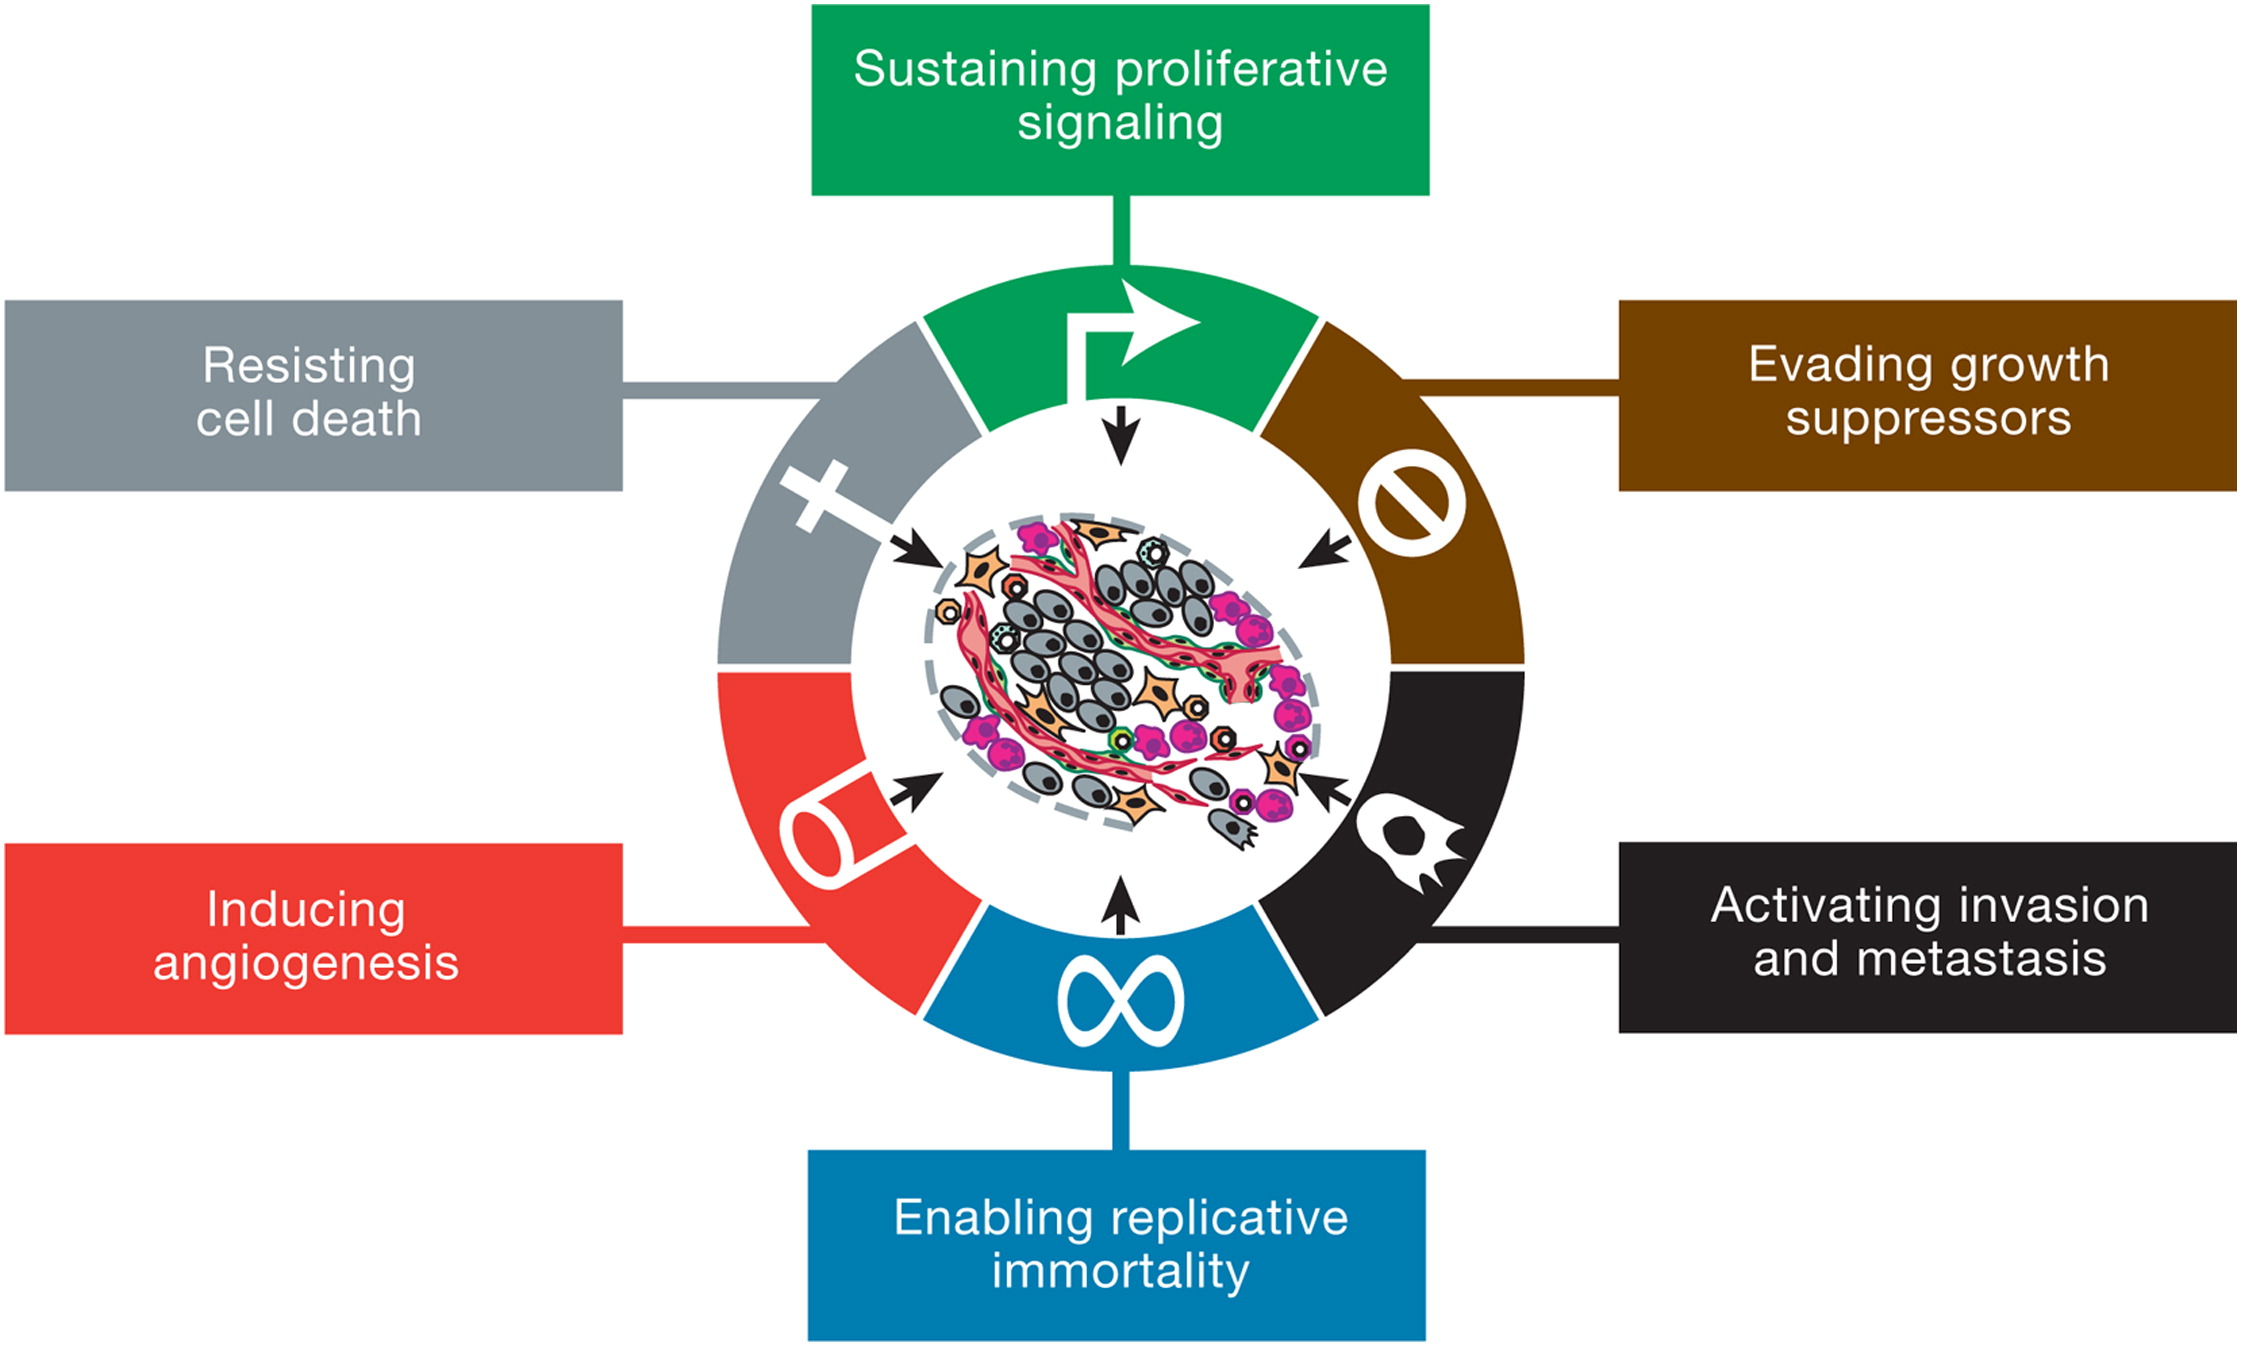
\includegraphics[width=.95\linewidth]{Figures/oldHallmarksCancer.jpg}
\caption[Original hallmarks of cancer]{Acquired capabilities of cancer; Functional capabilities acquired by most cancers during their development; Figure adapted from \protect\citeauthor*{Hanahan2000}\protect\cite{Hanahan2000}}\label{fig:oldhallmarks}
\end{figure}


These hallmarks were long considered the core of tumour development and the authors themselves hypothesised, that these core mechanics allow us to condense the complexity that cancer displays, both in the clinic as well as in labs, with a small set of rules, which all cancers have to obey \cite{Hanahan2000}. In their exact words: ``We foresee cancer research developing into a logical science, where the complexities of the disease, described in the laboratory and clinic, will become understandable in terms of a small number of underlying principles``

However, with 11 years of additional research into the topic, more hallmarks have been found and the original list was revised by the authors to contain additional characteristics, namely 
\begin{enumerate*}
\item Avoiding immune destruction
\item Tumour-promoting inflamation
\item Genome instability and mutation
\item Deregulating cellular energetics
\end{enumerate*}
(\autoref{fig:newhallmarks}) \cite{Hanahan2011}. And even then a few years later, even more hallmarks e.g. metabolic rewiring are now considered a part of the characteristics of cancer \cite{Fouad2017}.

\begin{figure}[!ht]
\centering
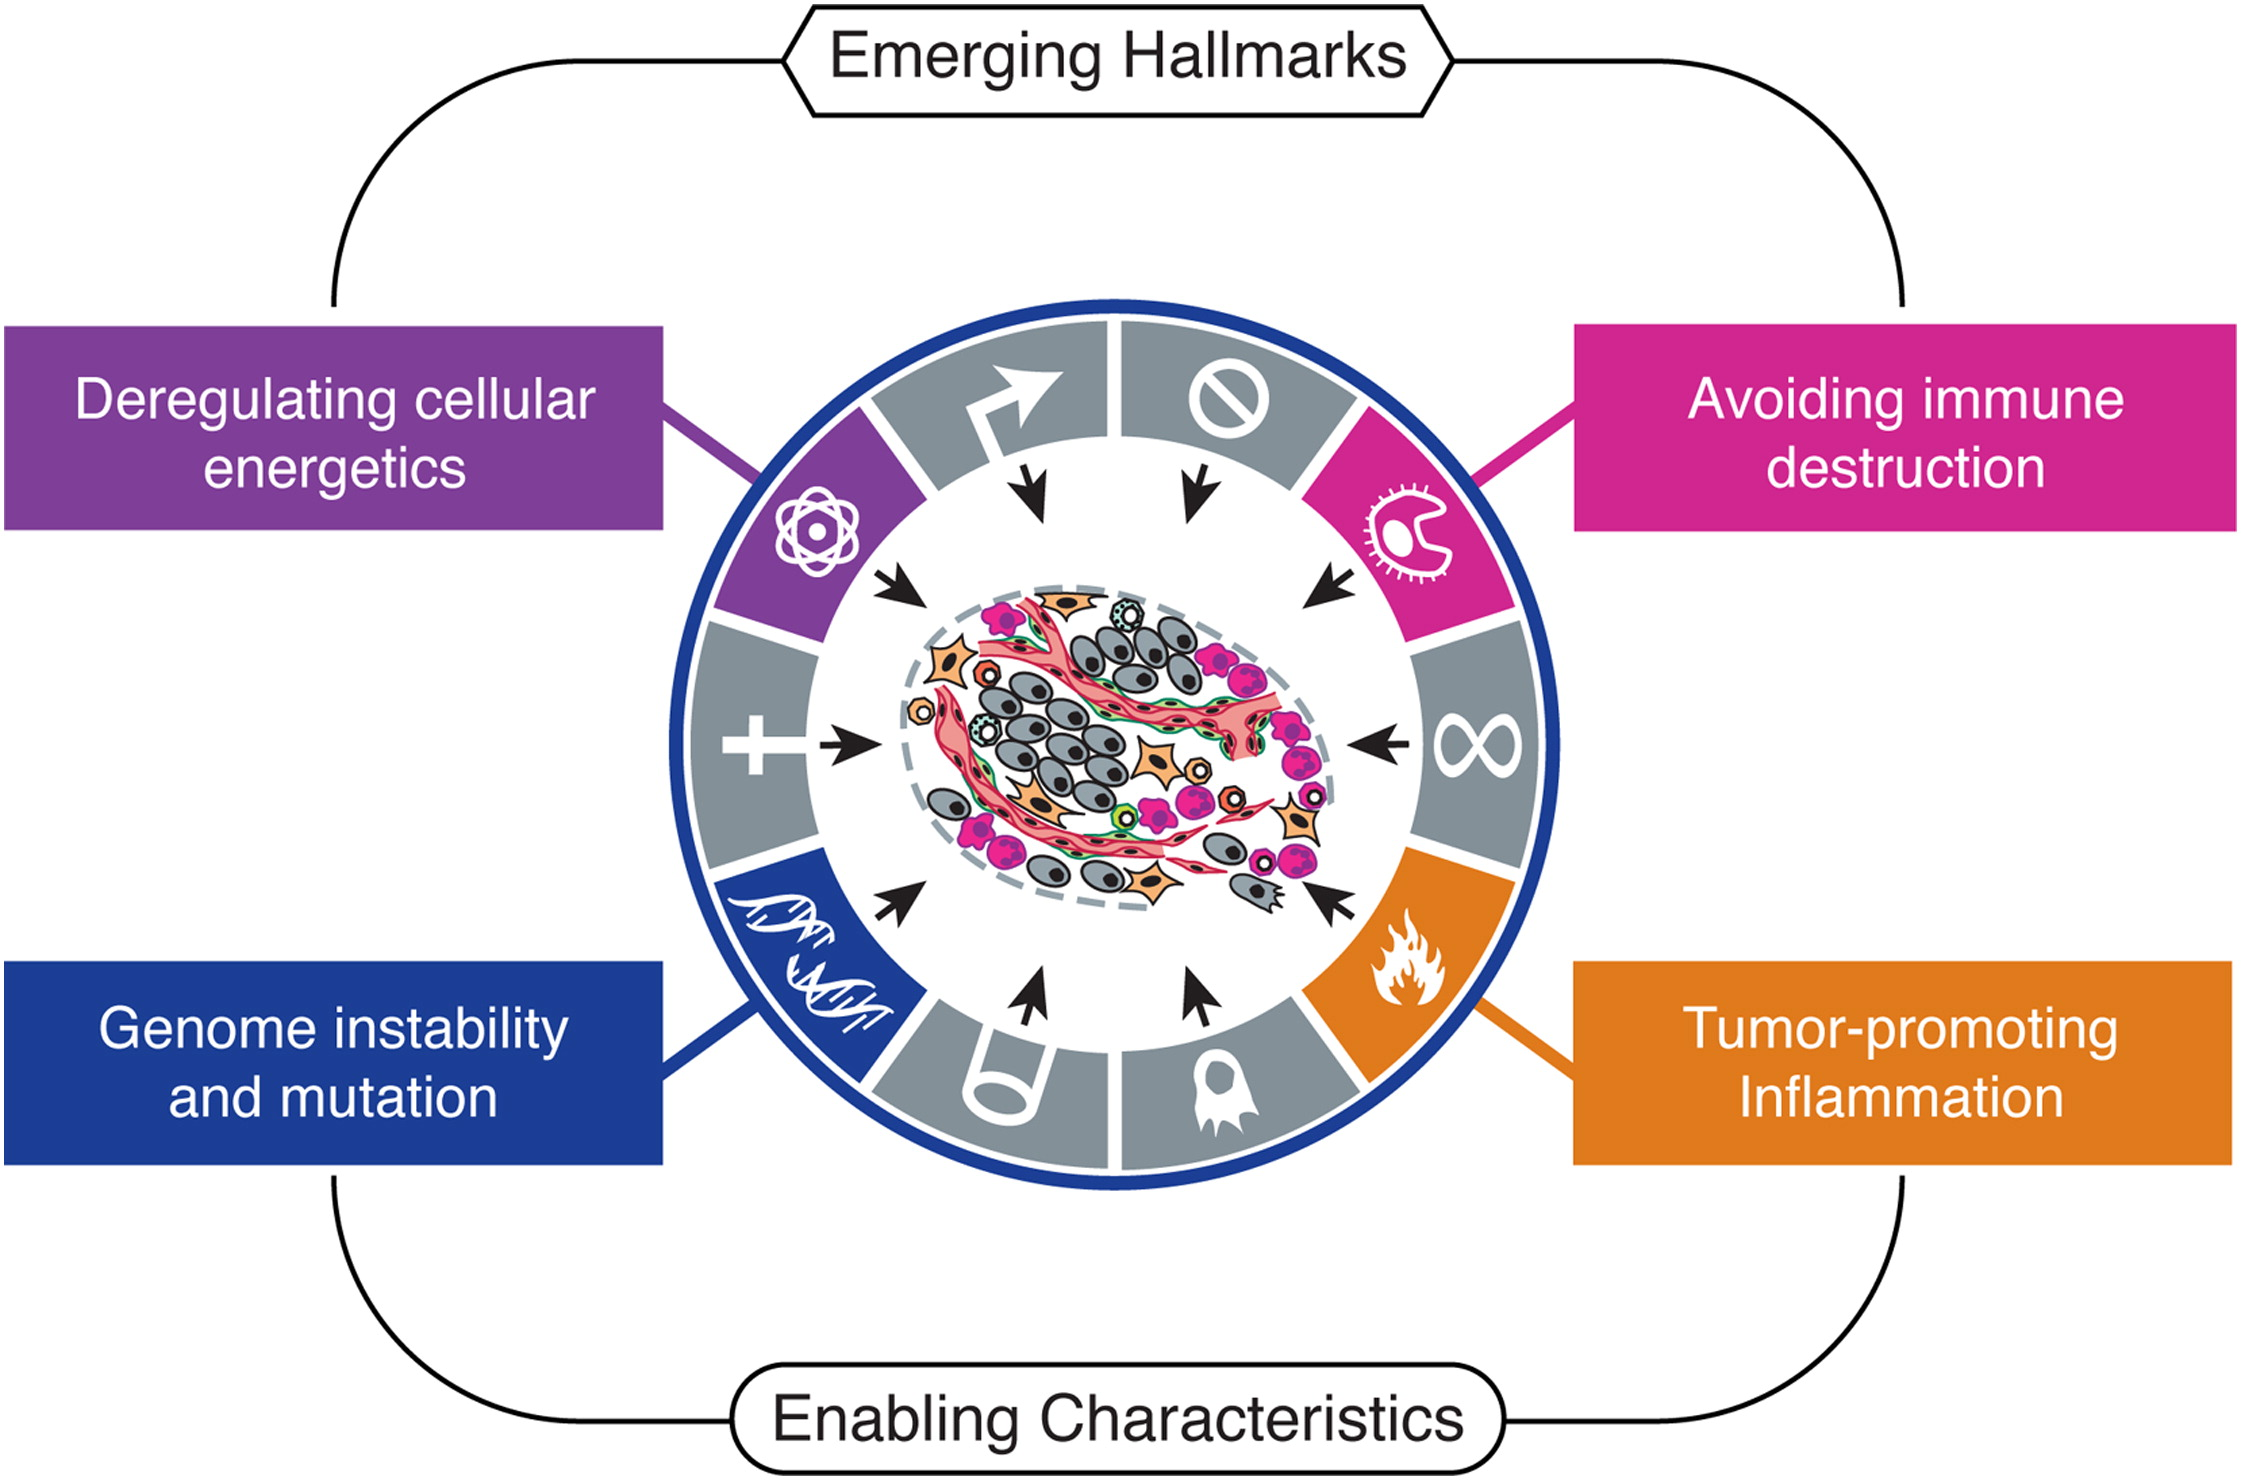
\includegraphics[width=.95\linewidth]{Figures/newHallmarksCancer.jpg}
\caption[New hallmarks of cancer]{Emerging hallmarks and enabling characteristics of cancer; updated version of the hallmarks figure (\autoref{fig:oldhallmarks}) with ; Figure adapted from \protect\citeauthor*{Hanahan2011}\protect\cite{Hanahan2011}}\label{fig:newhallmarks}
\end{figure}

So while the original set of the hallmarks was not sufficient or complete, it offered a good attempt at abstraction of biological concepts to describe cancers. In the following pages, I will outline each of those hallmarks and how it influences my research.

\todo[inline, color=red]{describe the hallmarks}

\subsubsection{Sustaining proliferative signaling - there are no breaks on the train}

\subsubsection{Evading growth suppressors}

\subsubsection{Activating invasion and metastasis - look at me... I am the organism now}

\subsubsection{Enabling replicative immortality}

\subsubsection{Inducing angiogenesis}

\subsubsection{Resisting cell death}

\subsection{Lungcancer}
\label{intro-sec:lungcancer}

With around 1.6 million deaths world-wide each year, lung cancer is the number one cause of cancer death \cite{Siegel2018}. Every year about twelve thousand Australians get diagnosed with lung cancer. These cases can be generally split into two groups: small cell lung cancers (SCLC) and non-small cell lung cancers (NSCLC), which account for around 15\% and 85\% of cases, respectively. The majority of NSCLC are either lung adenocarcinoma or lung squamous cell carcinoma \cite{Molina2008}. Even though smoking is highly associated with lung cancers, there is a big group of never smokers, with a high risk of lung cancers in East Asia, especially women, which is correlated with outside influences like pollution and occupational carcinogens and paired with genetic susceptibility \cite{Sun2007}.
This group usually shows \textit{EGFR} (epidermal growth factor receptor) driven tumours. EGFR is a transmembrane receptor tyrosine kinase, which is usually only expressed in epithelial, mesenchymal, and neurogenic tissue, but its overexpression in other tissues is a hallmark of many human malignancies, not just NSCLC.

\todo[inline]{Possibly change this to cancer in general}

%% original abstract
%Approximately 50% of patients with non-small cell lung cancer (NSCLC) develop acquired resistance to EGFR tyrosine kinase inhibitors (TKIs) through mutations in EGFR T790M. Maintaining a dynamic balance between T790M positive and negative clones offers an opportunity to delay the emergence of resistance and improve disease outcomes. It is now possible to quantify EGFR mutations using circulating tumour DNA (ctDNA) which can provide a surrogate measure of clonal populations within tumours. This project will utilise next generation sequencing (NGS) of tumour tissue and ctDNA in patients treated with EGFR TKIs to study clonal evolution patterns and predict optimal treatment approaches to delay therapeutic resistance.